\section{Overview}
	The DoodleBot was designed to the Project Requirements, Project Scope and Performance Indicators introduced in Chapter ~\ref{ch:intro}. An overall system architecture was designed as shown in Figure ~\ref{fig:system}. Once appropriate data types were chosen, each module of the system could be designed and tested in isolation. 
	
	This chapter will explore the engineering designs and decision that are core to DoodleBot project. The actual implementation of these designs are covered in chapter ~\ref{ch:implementation}.

\begin{figure}[h]
\centering
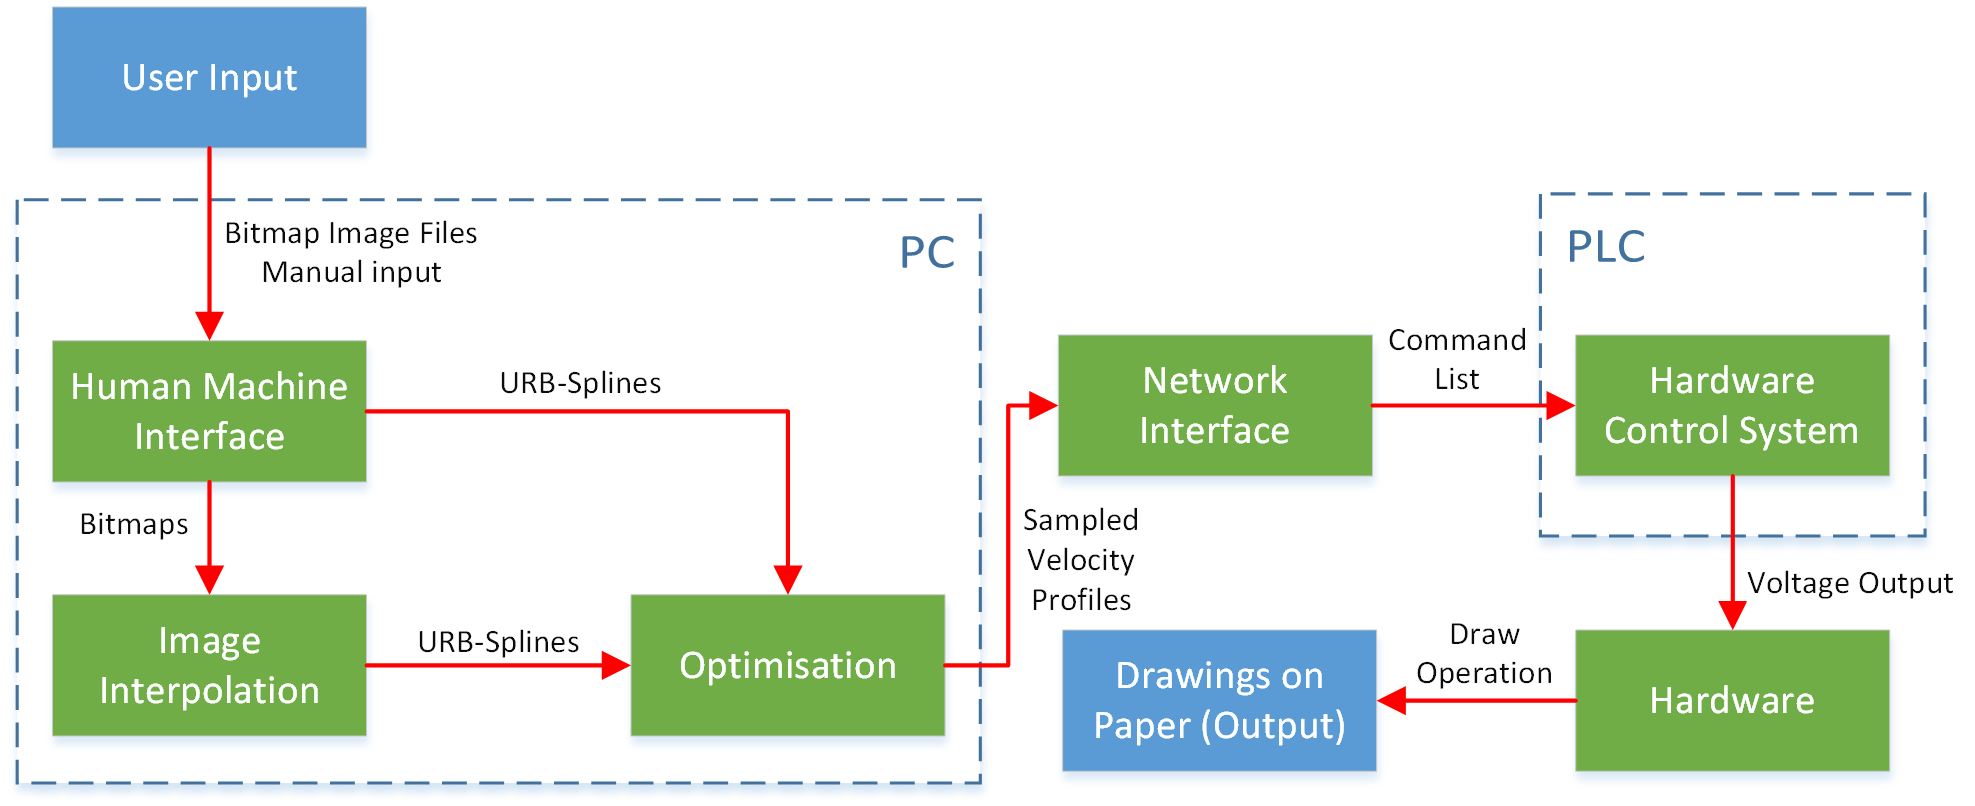
\includegraphics[width=0.9\textwidth]{figures/systemDesign/overview.png}
\caption{Modules and data flow of the DoodleBot system}
\label{fig:system}
\end{figure}

\subsection{Modules and Components}
	\subsubsection*{Input}
		The requirements stipulate a user being able to provide the machine input with photos or images. The DoodleBot was designed to accept any bitmap format (including compressed formats such as JPEG or PNG), but was optimized for simple images such as logos and photos of simple photographs with simple, distinct objects (such as buildings or hand drawn sketches on paper/whiteboards).
		
		In addition to this, the DoodleBot provides the added functionality of allowing the user to define URB-Splines directly through the Human-Machine Interface Interface.
		
	\subsubsection*{Output}
		The required output is a representation of the input to be drawn onto paper in a single colour via the DoodleBot mechanical hardware.
		
	\subsubsection*{Human-Machine Interface (HMI)} 
		The Human-Machine Interface (HMI) is the only way for a user to interact with the DoodleBot system and features an simple interface that includes the capability to provide both methods of input - selecting bitmap image files stored on the computer and a way to intuitively construct URB-Splines. Another important feature would be a way to control various parameters used in the optimisation process for testing purposes.
		
	\subsubsection*{Quadratic URB-Splines}
		The quadratic Uniform Rational Basis Spline (URBS) was chosen as the data type into the optimisation section. It is a versatile way of representing various curves with very little data and is defined by mathematical equations that are convenient for the optimisation calculations. See Section ~\ref{sec:design-urbs}.
		
	\subsubsection*{Image to Spline Interpolation}
		The Image to spline interpolation module takes the bitmap image input to the DoodleBot and generates a representation of the input in terms of Quadratic URB-Splines for use by the optimisation module. This module is what generates the reference image that the hardware tries to ultimately draw onto the paper (ie, the output). See Section ~\ref{sec:design-interpolation}.
		
	\subsubsection*{Optimisation}
		Two of the performance indicators identified in Chapter ~\ref{ch:intro} were related to how fast and how accurate the device can draw the image onto the output medium. The Optimisation module takes the input URB-Splines and generates velocity profiles (for use in the Hardware Control module) that are time optimal for given hardware constraints. See Section ~\ref{sec:design-optimisation}.

	\subsubsection*{Network Interface}
		One of the requirements of the project was to construct a network interface between the Programmable Logic Controller and the PC using an Ethernet connection. The network interface allows the sampled velocity profiles to be sent from the PC to PLC and includes software on both devices. 

	\subsubsection*{Hardware Control System}
		The Hardware Control System takes sampled velocity profiles for each axis and drives the two motors to match these profiles. The Hardware Control System also controls the two-state control of the Z-axis (draw functionality). Project requirements stipulated this module to be implemented on the Programmable Logic Controller. See Section ~\ref{sec:design-control}.